% =====================================================================
% ISW 2026 SUBMISSION (2-4 page abstract)
% Paste this into the LNCS Overleaf template (main.tex):
%   https://www.overleaf.com/latex/templates/springer-lecture-notes-in-computer-science/kzwwpvhwnvfj
% Upload the four .pdf figures (fig_imputation, fig_pca, fig_contingency,
% fig_loadings) into the Overleaf project and compile with pdflatex.
% =====================================================================

\documentclass[runningheads]{llncs}

\usepackage[T1]{fontenc}
\usepackage{graphicx}
\usepackage{booktabs}
\usepackage{amsmath}
\usepackage{amssymb}
\usepackage{caption}
\usepackage{url}
\usepackage{hyperref}

\begin{document}

\title{Unsupervised Discovery of Child Welfare Archetypes Across the African Union.}

\titlerunning{Child Welfare Profiles in Africa}

\author{Samuel Babalola\inst{*}}
\authorrunning{S. Babalola}

\institute{Faculty of Software Engineering, African Leadership University,
Kigali, Rwanda \\
\email{s.babalola@alustudent.com}}

\maketitle

\begin{abstract}
The African Union groups its 55 member states into eight Regional Economic Communities (RECs) for policy coordination, but it is unclear whether these geographic-political blocs reflect the underlying child welfare conditions they are meant to address. Using the 2026 \emph{Africa's Children Statistical Compendium} (UNICEF), we apply unsupervised pattern recognition over 257 indicators spanning mortality, nutrition, education, WASH, child protection, gender, and economic dimensions. We make two contributions. First, we benchmark six imputation methods on a held-out 15\% of known cells and find that low-rank matrix factorization achieves a 17\% lower standardized RMSE than a column-mean baseline; the standard iterative (MICE) imputer fails in this small-$n$/large-$p$ regime ($n=52$, $p=257$). Second, we apply PCA followed by $k$-means, hierarchical (Ward), and Gaussian-mixture clustering, recovering four stable archetypes of child welfare. Bootstrap analysis shows strong reproducibility (within-cluster co-assignment 0.70 vs.\ 0.13 between). The partition agrees only weakly with REC membership (Adjusted Rand Index $0.10$, NMI $0.23$), indicating that policy-coordination blocs and child welfare realities are largely orthogonal.

\keywords{Pattern recognition \and Unsupervised clustering \and Matrix factorization \and Imputation \and Child welfare \and Africa}
\end{abstract}

\section{Introduction}\label{sec:intro}

The African Union (AU) coordinates its 55 member states largely through eight Regional Economic Communities (RECs) -- ECOWAS, SADC, COMESA, EAC, ECCAS, AMU, IGAD, and CEN-SAD -- designed around trade, geography, and post-colonial alignments. Substantial child welfare resources are allocated and benchmarked along REC lines~\cite{ref_unicef_compendium,ref_au_recs}, with the implicit assumption that countries within a REC face sufficiently similar conditions for shared policies to be effective. To our knowledge this assumption has not been tested over the full breadth of child welfare indicators -- most existing analyses proceed indicator by indicator or rely on a-priori composite indices. We instead treat AU member states as points in a high-dimensional indicator space and ask: \emph{what natural archetypes of child welfare emerge from the data, and to what extent do these coincide with REC membership?} We contribute (i) a controlled benchmark of six imputation methods on the compendium's missingness pattern, including a low-rank matrix factorization tailored to the small-$n$/large-$p$ regime, and (ii) a clustering analysis using three independent algorithms with bootstrap stability and external validation against REC labels via ARI and NMI.

\section{Data and Methods}\label{sec:methods}

\paragraph{Data.} We use the 2026 \emph{Africa's Children Statistical Compendium}~\cite{ref_unicef_compendium}, which aggregates indicators across 21 thematic tables. Source datasets include UNICEF MICS, DHS, WHO modelled estimates, UNESCO UIS, and ILO labour data, with cut-off dates up to April 2026. After parsing multi-row headers and removing regional aggregates, we obtain a country-by-indicator matrix of 52 AU member states and 325 non-empty indicators (overall missingness 25.6\%). Restricting to indicators with $\leq 50\%$ missing values yields the working matrix $\mathbf{X} \in \mathbb{R}^{52 \times 257}$ with 14.4\% missingness. REC membership was assigned a single primary label per country: ECOWAS (15), COMESA (14), ECCAS (7), EAC (6), AMU (5), SADC (5).

\paragraph{Imputation benchmark.} Let $\Omega$ be the set of observed cells. We hide a random subset $\Omega_{\text{hold}} \subset \Omega$ of size $0.15|\Omega|$, apply each imputer, and report the standardized RMSE
\begin{equation}
\text{RMSE}_{\text{std}} = \sqrt{ \tfrac{1}{|\Omega_{\text{hold}}|} \sum_{(i,j) \in \Omega_{\text{hold}}} \!\big( (\hat{x}_{ij} - x_{ij}) / \sigma_j \big)^{2} },
\end{equation}
where $\sigma_j$ is the standard deviation of column $j$ on still-known cells. We average over $T=5$ random splits and compare column mean, column median, $k$-NN ($k\in\{5,10\}$), iterative chained-equations imputation~\cite{ref_mice}, and a low-rank matrix factorization (rank $r=5$) optimised by gradient descent on observed entries with Frobenius regularization~\cite{ref_mf}.

\paragraph{Clustering.} After imputation we standardize features and apply PCA, retaining 10 components ($73.4\%$ variance). We cluster in this space using $k$-means (50 restarts), Ward hierarchical clustering, and a Gaussian mixture. We choose $K=4$ to balance silhouette quality with the constraint $K \geq 4$ for meaningful comparison against the six RECs. Stability is estimated via $B=50$ bootstrap resamples; we report mean within- and between-cluster co-assignment probability. Agreement with REC labels is measured with Adjusted Rand Index (ARI)~\cite{ref_ari} and Normalized Mutual Information (NMI).

\section{Results}\label{sec:results}

\paragraph{Imputation.} Table~\ref{tab:imp} reports RMSE$_{\text{std}}$ across $T=5$ trials. Matrix factorization achieves $0.913 \pm 0.018$, a 16.6\% reduction over the column-mean baseline. $k$-NN underperforms the mean baseline -- with only $n{=}52$ rows, neighbourhoods are noisy. The iterative imputer fails (RMSE 4.55): per-column conditional regressions are ill-posed when $p > n$, and predictions diverge over iterations. This is itself informative: standard iterative methods popular in epidemiology are not directly applicable to compendium-style data without strong feature pre-selection.

\begin{figure}[t]
\centering
\begin{minipage}[c]{0.46\linewidth}
\centering
\captionof{table}{Imputation benchmark on 15\% held-out cells, 5 random splits.}\label{tab:imp}
\small\setlength{\tabcolsep}{4pt}
\begin{tabular}{lcc}
\toprule
Method & RMSE$_{\text{std}}$ & Std \\
\midrule
Column mean             & 1.101 & 0.027 \\
Column median           & 1.142 & 0.022 \\
$k$-NN ($k{=}5$)        & 1.183 & 0.034 \\
$k$-NN ($k{=}10$)       & 1.132 & 0.032 \\
Iterative (MICE)        & 4.553 & 0.241 \\
\textbf{Matrix fact.}   & \textbf{0.913} & \textbf{0.018} \\
\bottomrule
\end{tabular}
\end{minipage}\hfill
\begin{minipage}[c]{0.50\linewidth}
\centering
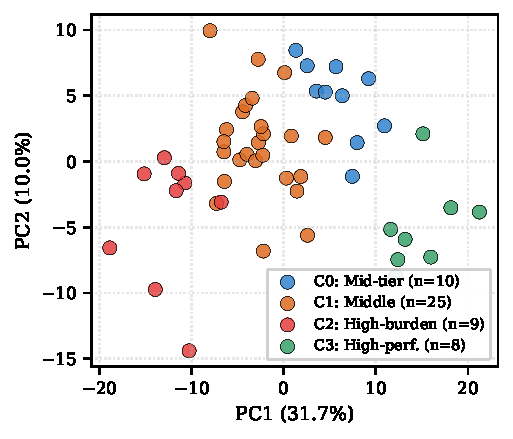
\includegraphics[width=\linewidth]{fig_pca_compact.pdf}
\captionof{figure}{PCA of the 52 AU states, coloured by data-driven cluster.}\label{fig:pca}
\end{minipage}
\end{figure}

\paragraph{Cluster structure.} The three clustering algorithms agree well (pairwise ARI 0.42--0.68), indicating the structure is intrinsic rather than algorithm-specific. Bootstrap stability for $k$-means is high: within-cluster co-assignment 0.704 vs.\ between-cluster 0.128 (gap $0.576$). Figure~\ref{fig:pca} shows the four archetypes in the PC1--PC2 plane (capturing $41.7\%$ of variance); the same projection coloured by REC (not shown) shows the REC labels disperse across cluster boundaries.

The four archetypes are: \textbf{C3 -- High-performance} ($n{=}8$, AMU members plus Cabo Verde, Mauritius, Seychelles -- low under-five mortality, high WASH, low fertility); \textbf{C0 -- Mid-tier} ($n{=}10$, mostly Southern and East African states); \textbf{C1 -- Middle} ($n{=}25$, a large mid-development group spanning West and East Africa); \textbf{C2 -- High-burden} ($n{=}9$: Chad, DRC, Eritrea, Ethiopia, Niger, Nigeria, Somalia, South Sudan, Sudan -- highest under-five and adolescent mortality, lowest WASH).

\paragraph{Comparison with RECs.} The data-driven partition agrees only weakly with REC membership: ARI is $0.104$ ($k$-means), $0.124$ (hierarchical), $0.126$ (GMM); NMI ranges from $0.227$ to $0.267$. Inspection of the contingency (Table~\ref{tab:cont}) shows that AMU is the only REC concentrated in a single archetype; all other RECs spread across three or four. ECOWAS distributes its 15 members across all four archetypes, and the high-burden archetype draws members from four different RECs.

\begin{table}[t]
\caption{Cluster--REC contingency.}\label{tab:cont}
\centering\small\setlength{\tabcolsep}{6pt}
\begin{tabular}{lcccccc}
\toprule
Cluster & AMU & COMESA & EAC & ECCAS & ECOWAS & SADC \\
\midrule
High-burden     & 0 & 4 & 1 & 2 & 2 & 0 \\
High-performance& 4 & 3 & 0 & 0 & 1 & 0 \\
Mid-tier        & 0 & 3 & 2 & 2 & 0 & 3 \\
Middle          & 1 & 4 & 3 & 3 & 12 & 2 \\
\bottomrule
\end{tabular}
\end{table}

\section{Discussion and Conclusion}\label{sec:discussion}

The principal empirical finding is the disconnect between REC membership and data-driven child welfare archetypes (ARI $\approx 0.1$). RECs were designed for economic integration, not pediatric outcomes; the magnitude of disagreement, however, has not previously been quantified. Comparative benchmarking along REC lines may therefore obscure the true peer set for any given country: a low-mortality and a high-mortality COMESA country face fundamentally different programming challenges. The high-burden archetype unites countries facing protracted humanitarian crisis (South Sudan, Somalia, Sudan, DRC) regardless of REC affiliation, where coordination on common challenges may be more impactful than within-REC coordination.

\paragraph{Limitations and conclusion.} The compendium is a snapshot; longitudinal extension is the natural next step. With $n{=}52, p{=}257$ the regime is small-$n$/high-$p$, motivating our use of unsupervised methods and stability metrics; supervised modelling here must be approached cautiously. We recovered four stable archetypes of child welfare across the African Union with clear, interpretable indicator profiles. Methodologically, low-rank matrix factorization is well-suited to compendium-style data, materially outperforming column-mean and iterative chained-equations baselines. The archetypes show only weak agreement with the RECs (ARI $\approx 0.10$), suggesting data-driven peer groupings could complement geographically-defined coordination blocs for child welfare programming.

\begin{thebibliography}{5}\small
\bibitem{ref_unicef_compendium}
UNICEF: Africa's Children 2026 Statistical Compendium. UNICEF Data Division (2026)

\bibitem{ref_au_recs}
African Union: Regional Economic Communities. \url{https://au.int/en/organs/recs}

\bibitem{ref_mice}
van Buuren, S., Groothuis-Oudshoorn, K.: mice: Multivariate Imputation by Chained Equations in R. J. Stat.\ Softw.\ 45(3), 1--67 (2011)

\bibitem{ref_mf}
Cand\`es, E.J., Recht, B.: Exact matrix completion via convex optimization. Found.\ Comput.\ Math.\ 9(6), 717--772 (2009)

\bibitem{ref_ari}
Hubert, L., Arabie, P.: Comparing partitions. J. Classif.\ 2(1), 193--218 (1985)
\end{thebibliography}

\end{document}
